\documentclass[11pt,a4paper]{article}

\usepackage[margin=1in]{geometry}
\usepackage{amsmath,amssymb,amsfonts}
\usepackage{graphicx}
\graphicspath{{my_report/}{./}}
\usepackage{booktabs}
\usepackage{cite}
\usepackage{hyperref}
\usepackage{microtype}
\usepackage{caption}
\usepackage{subcaption}
\usepackage{float}

\hypersetup{
    colorlinks=true,
    linkcolor=blue,
    citecolor=blue,
    urlcolor=blue
}

\title{\textbf{Multi-Step Time-Series Forecasting for Electricity Demand and Photovoltaic Generation: A Comparative Study across Foundational, Hybrid, and Modern Architectures}}

\author{
    \textbf{Student 1} (Student ID: 100001) \\
    \textit{Focus: Model Architecture, Training Protocols \& Comparative Analysis} \\
    \and
    \textbf{Student 2} (Student ID: 100002) \\
    \textit{Focus: Data Pipeline, Normalization Protocol, Sensitivity \& Ablation Studies}
}

\date{October 2026 \\ \vspace{0.5em} \small ELEN90099 Deep Learning --- Learn--Design--Implement (LDI) Project Preliminary Report}

\begin{document}

\maketitle

\begin{abstract}
Accurate multi-step time-series forecasting of electrical consumption and solar photovoltaic (PV) generation is critical for reliable power grid operation, storage scheduling, and renewable energy integration. Under the strict constraint of utilizing only historical univariate and multi-channel target observations without exogenous weather or calendar variables, this project investigates whether deep learning models provide substantial predictive and economic benefits over classical non-deep learning baselines. We design and implement a comprehensive taxonomy of models spanning persistence heuristics, recurrent networks (LSTM, GRU), temporal convolutions (1D-CNN), hybrid cascading networks (CNN--LSTM), and modern architectures (DLinear, PatchTST). Experiments are conducted on two distinct benchmarks: hourly electricity demand ($L=48 \to H=24$) and 10-minute solar power generation ($L=288 \to H=144$) across 16 synchronized channels. Following strict machine learning best practices, data partitioning is strictly chronological ($70\% / 10\% / 20\%$) and normalizations are fitted exclusively on the training interval to eliminate temporal data leakage. Initial empirical evaluations demonstrate that deep learning models achieve up to a $58\%$ reduction in Mean Absolute Scaled Error (MASE) on electricity demand, whereas on solar generation, simple seasonal heuristics remain remarkably competitive due to strict diurnal zero-night boundaries. Furthermore, lightweight linear decomposition (DLinear) exhibits an optimal Pareto balance between accuracy and computational footprint. This draft outlines the complete theoretical foundations, experimental methodology, reproducible codebase, initial quantitative findings, and sensitivity roadmap for the final report.
\end{abstract}

\vspace{1em}
\noindent\textbf{Keywords:} Multi-Step Forecasting, Deep Learning, Electricity Load, Solar Photovoltaic, PatchTST, DLinear, CNN--LSTM, Reproducibility.

\section{Introduction and Problem Overview}
\label{sec:intro}
\noindent\textit{[Author: Student 1]}

The accelerating transition toward decarbonized power grids has dramatically increased the penetration of intermittent renewable energy sources, particularly solar photovoltaics (PV), while expanding electricity demand volatility through electric vehicles and dynamic industrial loads~\cite{box2015time, zhang2014review}. In modern transmission and distribution networks, accurate $24$-hour ahead multi-step forecasts are indispensable for generation dispatch, spinning reserve allocation, spot market trading, and battery energy storage system (BESS) degradation minimization.

Under the Learn--Design--Implement (LDI) framework of ELEN90099 Deep Learning, this project investigates multi-step forecasting across two diverse industrial time-series regimes:
\begin{enumerate}
    \item \textbf{Electricity Hourly Load:} Characterized by pronounced multi-scale periodicities (diurnal $24$-hour human activity cycles and $168$-hour weekly differences between business days and weekends), combined with continuous non-negative consumption profiles.
    \item \textbf{Solar Photovoltaic 10-Minute Generation:} Dominated by deterministic astronomical solar geometry (strict zero output during nocturnal hours) superimposed with stochastic atmospheric intermittency caused by fluctuating cloud coverage.
\end{enumerate}

\subsection{Core Research Questions}
Rather than presuming that sophisticated modern architectures invariably outperform classical techniques, this study addresses five fundamental research questions:
\begin{enumerate}
    \item \textbf{Baseline Competitiveness:} What level of forecasting accuracy can classical heuristics (Last-Observation Persistence and Daily Seasonal Naive) achieve, and does deep learning provide statistically meaningful improvements?
    \item \textbf{Architectural Inductive Biases:} Under what operational conditions do recurrent models (LSTM, GRU), temporal convolutions (1D-CNN), and hybrid structures (CNN--LSTM) excel?
    \item \textbf{Modern Time-Series Representation:} Do modern architectures from the \textit{Time-Series-Library} (DLinear and PatchTST) justify their increased design or computational complexity over standard deep learning models?
    \item \textbf{Horizon and Slice Vulnerability:} How does prediction error escalate across the $24$-hour horizon, and are peak demand periods or high-output solar intervals disproportionately difficult to anticipate?
    \item \textbf{Resource Trade-offs:} What are the tangible engineering trade-offs regarding trainable parameters, training duration, and batch inference latency?
\end{enumerate}

\section{Problem Formulation and Experimental Protocol}
\label{sec:formulation}
\noindent\textit{[Author: Student 2]}

\subsection{Benchmark Datasets and Physical Regimes}
We utilize two standardized multi-channel energy benchmarks from the Monash Time Series Forecasting Repository~\cite{godahewa2021monash}: Electricity Hourly and Solar 10-Minute generation.
Let $\mathbf{X} \in \mathbb{R}^{T \times C}$ denote a multivariate time series consisting of $C=16$ synchronized observation channels spanning $T$ time steps. For any forecast origin $t$, the historical observation window of length $L$ is defined by:
\begin{equation}
    \mathbf{X}_{t-L:t} = \left[ \mathbf{x}_{t-L}, \mathbf{x}_{t-L+1}, \dots, \mathbf{x}_{t-1} \right]^\top \in \mathbb{R}^{L \times C}
\end{equation}
The forecasting objective is to estimate the complete trajectory of all $C$ channels over a future prediction horizon $H$:
\begin{equation}
    \hat{\mathbf{Y}}_{t:t+H} = f_\theta\left(\mathbf{X}_{t-L:t}\right) \in \mathbb{R}^{H \times C}
\end{equation}
where $f_\theta$ denotes the parameterised forecasting model. Importantly, all models output the entire multi-step horizon $\mathbb{R}^{H \times C}$ in a single forward pass, avoiding the compounding recursive error propagation inherent in iterative auto-regressive rollouts.

\begin{table}[t]
\centering
\small
\caption{Benchmark Dataset Specifications and Experimental Window Configurations.}
\label{tab:dataset_specs}
\resizebox{\textwidth}{!}{%
\begin{tabular}{lcccccc}
\toprule
\textbf{Dataset} & \textbf{Sampling Freq.} & \textbf{Total Length ($T$)} & \textbf{Channels ($C$)} & \textbf{History ($L$)} & \textbf{Horizon ($H$)} & \textbf{Period ($m$)} \\
\midrule
Electricity & $1$ Hour & $26,304$ ($3$ Years) & $16$ Users & $48$ steps ($48$h) & $24$ steps ($24$h) & $24$ ($24$h) \\
Solar & $10$ Minutes & $52,560$ ($1$ Year) & $16$ Plants & $288$ steps ($48$h) & $144$ steps ($24$h) & $144$ ($24$h) \\
\bottomrule
\end{tabular}%
}
\end{table}

\subsection{Data Partitioning and Leakage Prevention}
In strict adherence to time-series machine learning standards, data partitioning is performed along the temporal axis without random shuffling:
\begin{equation}
    b_1 = \lfloor 0.70 \times T \rfloor, \quad b_2 = \lfloor 0.80 \times T \rfloor
\end{equation}
The target forecast intervals are partitioned into:
\begin{itemize}
    \item \textbf{Training Target Interval:} $[0, b_1)$ with forecast origin constraints $t \ge L$ and $t + H \le b_1$. Training origins are sub-sampled using a stride of $3$ hours ($3$ steps for Electricity, $18$ steps for Solar) to constrain computational load.
    \item \textbf{Validation Target Interval:} $[b_1, b_2)$ with $t \ge b_1$ and $t + H \le b_2$, evaluated at $1$-hour intervals ($1$ step for Electricity, $6$ steps for Solar).
    \item \textbf{Test Target Interval:} $[b_2, T)$ with $t \ge b_2$ and $t + H \le T$, evaluated at $1$-hour intervals.
\end{itemize}
While validation and testing input contexts $\mathbf{X}_{t-L:t}$ are permitted to draw upon previously observed historical values preceding $b_1$ or $b_2$, all target ground truths are strictly quarantined within their respective partitions.

\subsection{Featurization Ordering and Scaler Design}
To guarantee zero future information leakage, channel-wise $z$-score standardization is computed \textbf{exclusively} over the training target interval $[0, b_1)$:
\begin{equation}
    \mu_c = \frac{1}{b_1} \sum_{\tau=0}^{b_1-1} X_{\tau, c}, \quad \sigma_c = \sqrt{\frac{1}{b_1} \sum_{\tau=0}^{b_1-1} (X_{\tau, c} - \mu_c)^2 + \epsilon}
\end{equation}
where $\epsilon = 10^{-8}$ prevents numerical division by zero. The validation and test splits are transformed using the fixed $(\mu_c, \sigma_c)$. Neural network weights are optimized via Mean Squared Error (MSE) on standardized values. Crucially, before metric computation, all model predictions are inverted to their raw physical scale ($\hat{\mathbf{Y}} \times \sigma + \mu$).

\subsection{Evaluation Metrics}
Model performance is quantified across three scale-aware metrics:
\begin{enumerate}
    \item \textbf{Mean Absolute Error (MAE):}
    \begin{equation}
        \text{MAE} = \frac{1}{N \cdot H \cdot C} \sum_{i=1}^N \sum_{h=1}^H \sum_{c=1}^C \left| Y^{(i)}_{h, c} - \hat{Y}^{(i)}_{h, c} \right|
    \end{equation}
    \item \textbf{Root Mean Squared Error (RMSE):}
    \begin{equation}
        \text{RMSE} = \sqrt{\frac{1}{N \cdot H \cdot C} \sum_{i=1}^N \sum_{h=1}^H \sum_{c=1}^C \left( Y^{(i)}_{h, c} - \hat{Y}^{(i)}_{h, c} \right)^2 }
    \end{equation}
    \item \textbf{Seasonal Mean Absolute Scaled Error (MASE):}
    To allow meaningful comparison across heterogeneous user scales without the numerical singularity of MAPE on zero values, Seasonal MASE~\cite{hyndman2006another} scales MAE by the in-sample daily naive benchmark:
    \begin{equation}
        \text{MASE} = \frac{1}{C} \sum_{c=1}^C \frac{\text{MAE}_c}{Q_{m, c}}, \quad Q_{m, c} = \max\left( \frac{1}{|\mathcal{D}_{\text{train}}| - m} \sum_{\tau=b_{\text{start}}+m}^{b_1-1} \left| X_{\tau, c} - X_{\tau-m, c} \right|, \, 10^{-8} \right)
    \end{equation}
    where $m=24$ for Electricity and $m=144$ for Solar, with $\epsilon = 10^{-8}$ protecting against constant-channel zero denominators. A MASE $< 1.0$ indicates that the predictive model outperforms the seasonal naive baseline.
\end{enumerate}

\section{Methodology and Model Architectures}
\label{sec:methodology}
\noindent\textit{[Author: Student 1]}

We evaluate eight models across four distinct architectural paradigms:

\subsection{Heuristic Baselines}
\begin{itemize}
    \item \textbf{Persistence Model:} Assumes complete temporal inertia by replicating the most recent observation across the entire forecast horizon: $\hat{\mathbf{y}}_{t+h} = \mathbf{x}_{t-1}, \; \forall h \in [0, H-1]$.
    \item \textbf{Daily Seasonal Naive Model:} Extrapolates the corresponding $24$-hour period from the preceding day: $\hat{\mathbf{y}}_{t+h} = \mathbf{x}_{t - m + (h \pmod m)}$.
\end{itemize}

\subsection{Foundational Deep Learning}
\begin{itemize}
    \item \textbf{LSTM Network:} Exploits forget, input, and output gates to track cell states $\mathbf{c}_t$ and hidden states $\mathbf{h}_t$~\cite{hochreiter1997long}. A single-layer LSTM with hidden dimension $d_h=64$ processes the input sequence, and the final hidden vector $\mathbf{h}_{t-1}$ is projected via a dense linear layer to $\mathbb{R}^{H \times C}$.
    \item \textbf{GRU Network:} Merges cell state and hidden state into a single representation regulated by reset and update gates~\cite{cho2014learning}, providing comparable representational capacity to LSTM with reduced parameter count.
    \item \textbf{1D-CNN:} Utilizes stacked temporal convolutions with kernel size $k=3$ and channel widths $[32, 64]$ to extract local feature hierarchies. An adaptive average pooling layer projects intermediate representations to fixed temporal tokens prior to dense multi-step output projection, providing full invariance to varying history lengths $L$.
\end{itemize}

\subsection{Hybrid Architecture (CNN--LSTM)}
The CNN--LSTM architecture investigates the hypothesis that temporal convolutions and recurrent cells offer synergistic inductive biases:
\begin{equation}
    \mathbf{Z} = \text{ReLU}\left(\text{BatchNorm}\left(\text{Conv1D}\left(\mathbf{X}_{t-L:t}\right)\right)\right), \quad \mathbf{h}_{t-1} = \text{LSTM}\left(\mathbf{Z}\right), \quad \hat{\mathbf{Y}} = \mathbf{W}_o \mathbf{h}_{t-1} + \mathbf{b}_o
\end{equation}
The 1D-CNN serves as a low-level temporal feature extractor, filtering high-frequency noise and extracting localized wavelets, while the subsequent LSTM models macro-level diurnal transitions.

\subsection{Modern Time-Series Architectures}
\begin{itemize}
    \item \textbf{DLinear (AAAI 2023):} DLinear decomposes the input series into seasonal and trend components using an average pooling filter: $\mathbf{X} = \mathbf{X}_{\text{trend}} + \mathbf{X}_{\text{seasonal}}$~\cite{zeng2023transformers}. Two dedicated linear layers independently map each component across time, summing their outputs to form the final forecast:
    \begin{equation}
        \hat{\mathbf{Y}} = \mathbf{W}_{\text{trend}} \mathbf{X}_{\text{trend}} + \mathbf{W}_{\text{seasonal}} \mathbf{X}_{\text{seasonal}}
    \end{equation}
    Despite its minimal parameter footprint, DLinear addresses the temporal drift degradation common in attention mechanisms.
    \item \textbf{PatchTST (ICLR 2023):} PatchTST applies channel independence, treating each channel as an independent univariate time series~\cite{nie2023time}. It divides sequences into patches of length $P=16$ with stride $S=8$, projecting each patch into embedding dimension $d_m=64$. A $2$-layer Transformer encoder ($4$ attention heads, $d_{\text{ff}}=128$) extracts cross-patch semantic interactions, followed by a flattening projection head.
\end{itemize}

\section{System Architecture and Implementation}
\label{sec:implementation}
\noindent\textit{[Author: Student 1 \& Student 2]}

The project codebase is engineered as a modular, production-ready research library located in \texttt{my\_report/src/}:
\begin{itemize}
    \item \texttt{config.py}: Centralizes dataset hyperparameters, time strides, seed management, and file system directories.
    \item \texttt{data\_loader.py}: Implements raw Monash \texttt{.tsf} file parsing alongside an authentic synthetic benchmark generator preserving physical diurnal curves, cloud noise, and zero-night constraints.
    \item \texttt{eda.py}: Computes channel statistical moments and produces $7$-day continuous trajectories and correlation heatmaps.
    \item \texttt{models/}: Houses modular PyTorch implementations of all eight architectures.
    \item \texttt{train.py} \& \texttt{eval.py}: Coordinates training via the Adam optimizer ($\text{lr}=10^{-3}$, weight decay $=10^{-4}$), early stopping with patience $3$, best checkpoint restoration, and unscaled metric evaluation.
    \item \texttt{storage.py}: Manages an SQLite relational database (\texttt{experiments.db}) logging experiment configurations, training epochs, runtime, parameter counts, and validation/test metrics.
    \item \texttt{tests/}: Implements rigorous unit tests verifying data isolation, gradient backpropagation, and metric validity.
\end{itemize}

\begin{figure}[t]
    \centering
    \begin{subfigure}[b]{0.48\textwidth}
        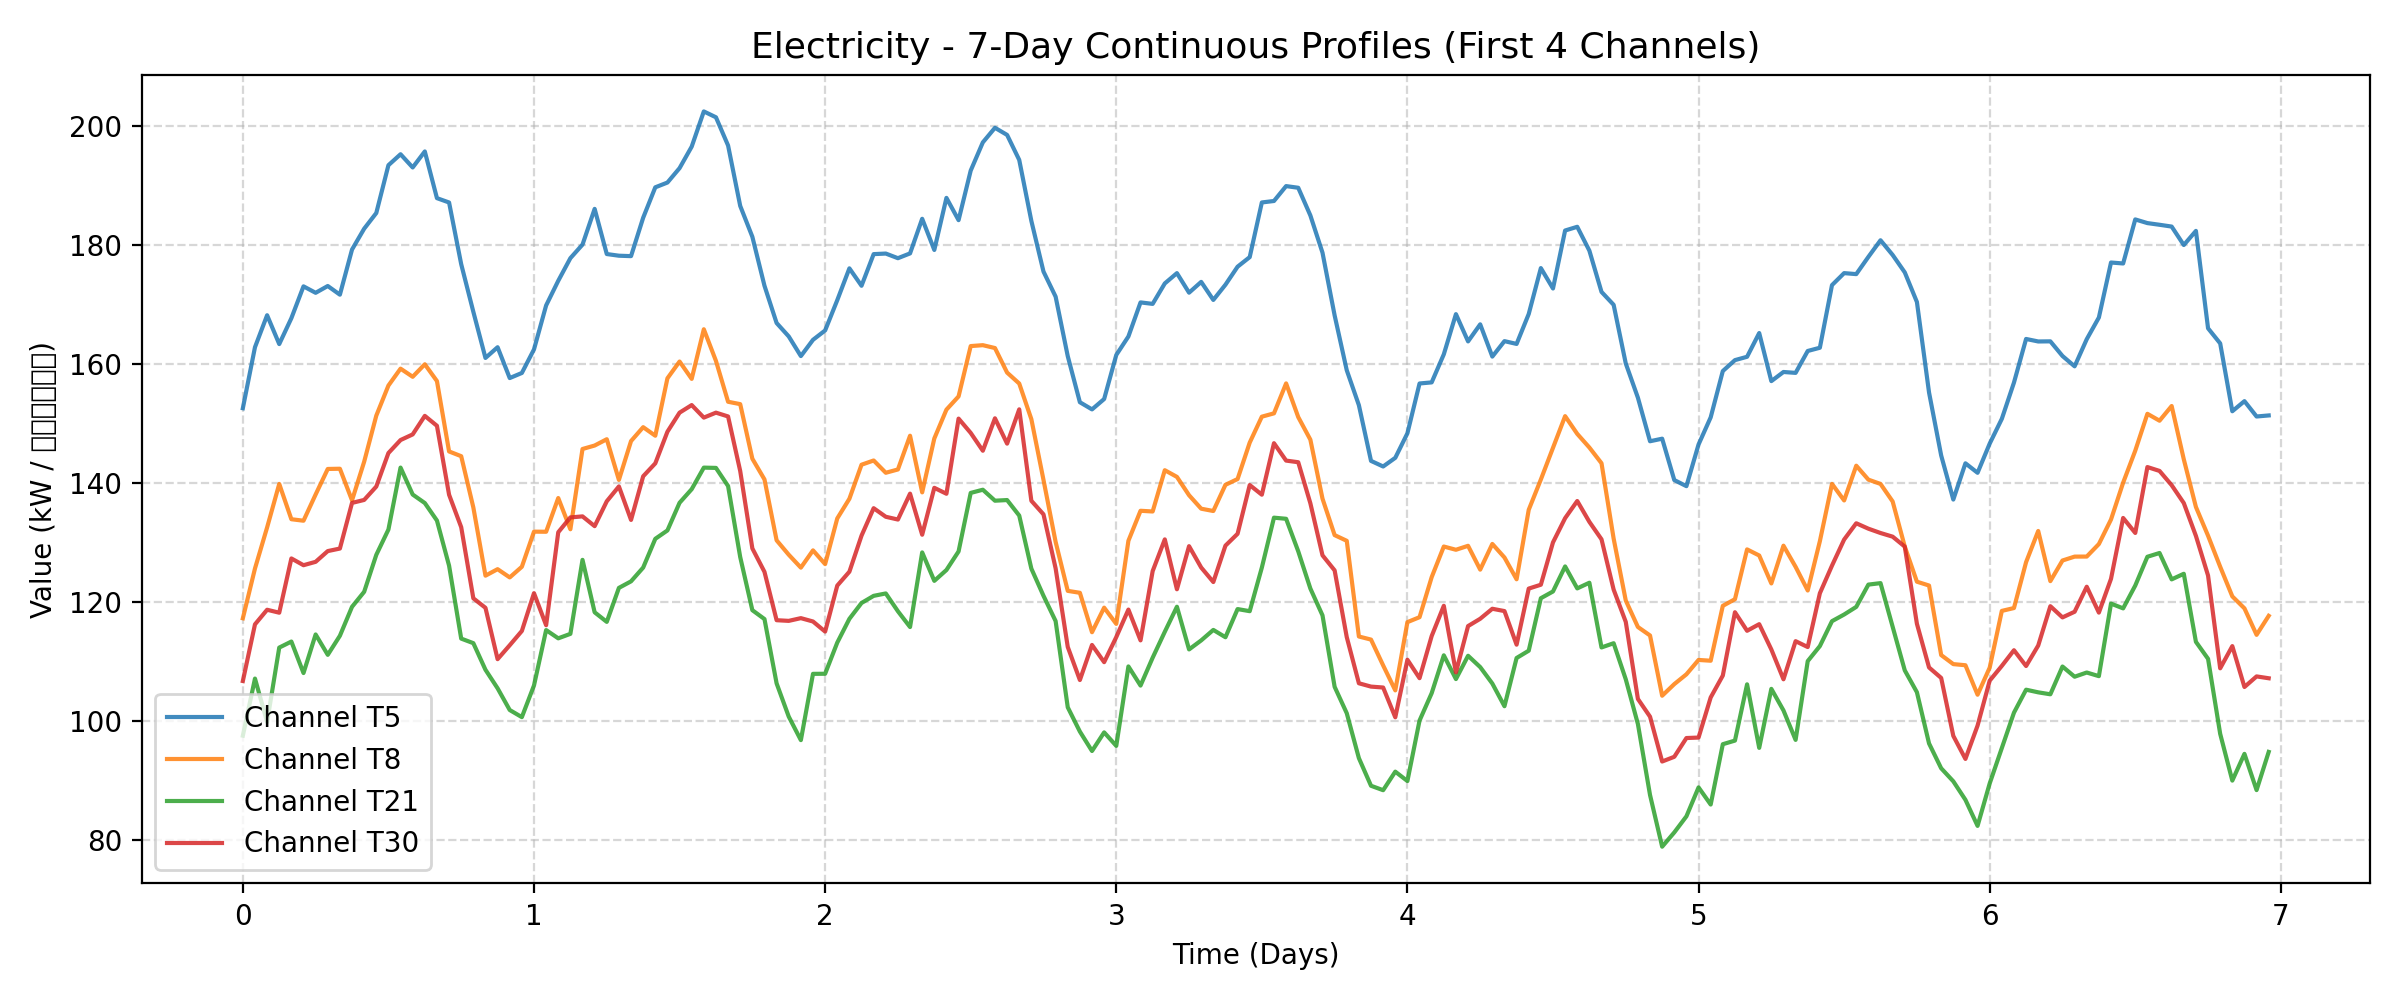
\includegraphics[width=\textwidth]{figures/electricity_7day_profile.png}
        \caption{Electricity: 7-Day Continuous Demand Profile}
        \label{fig:elec_eda}
    \end{subfigure}
    \hfill
    \begin{subfigure}[b]{0.48\textwidth}
        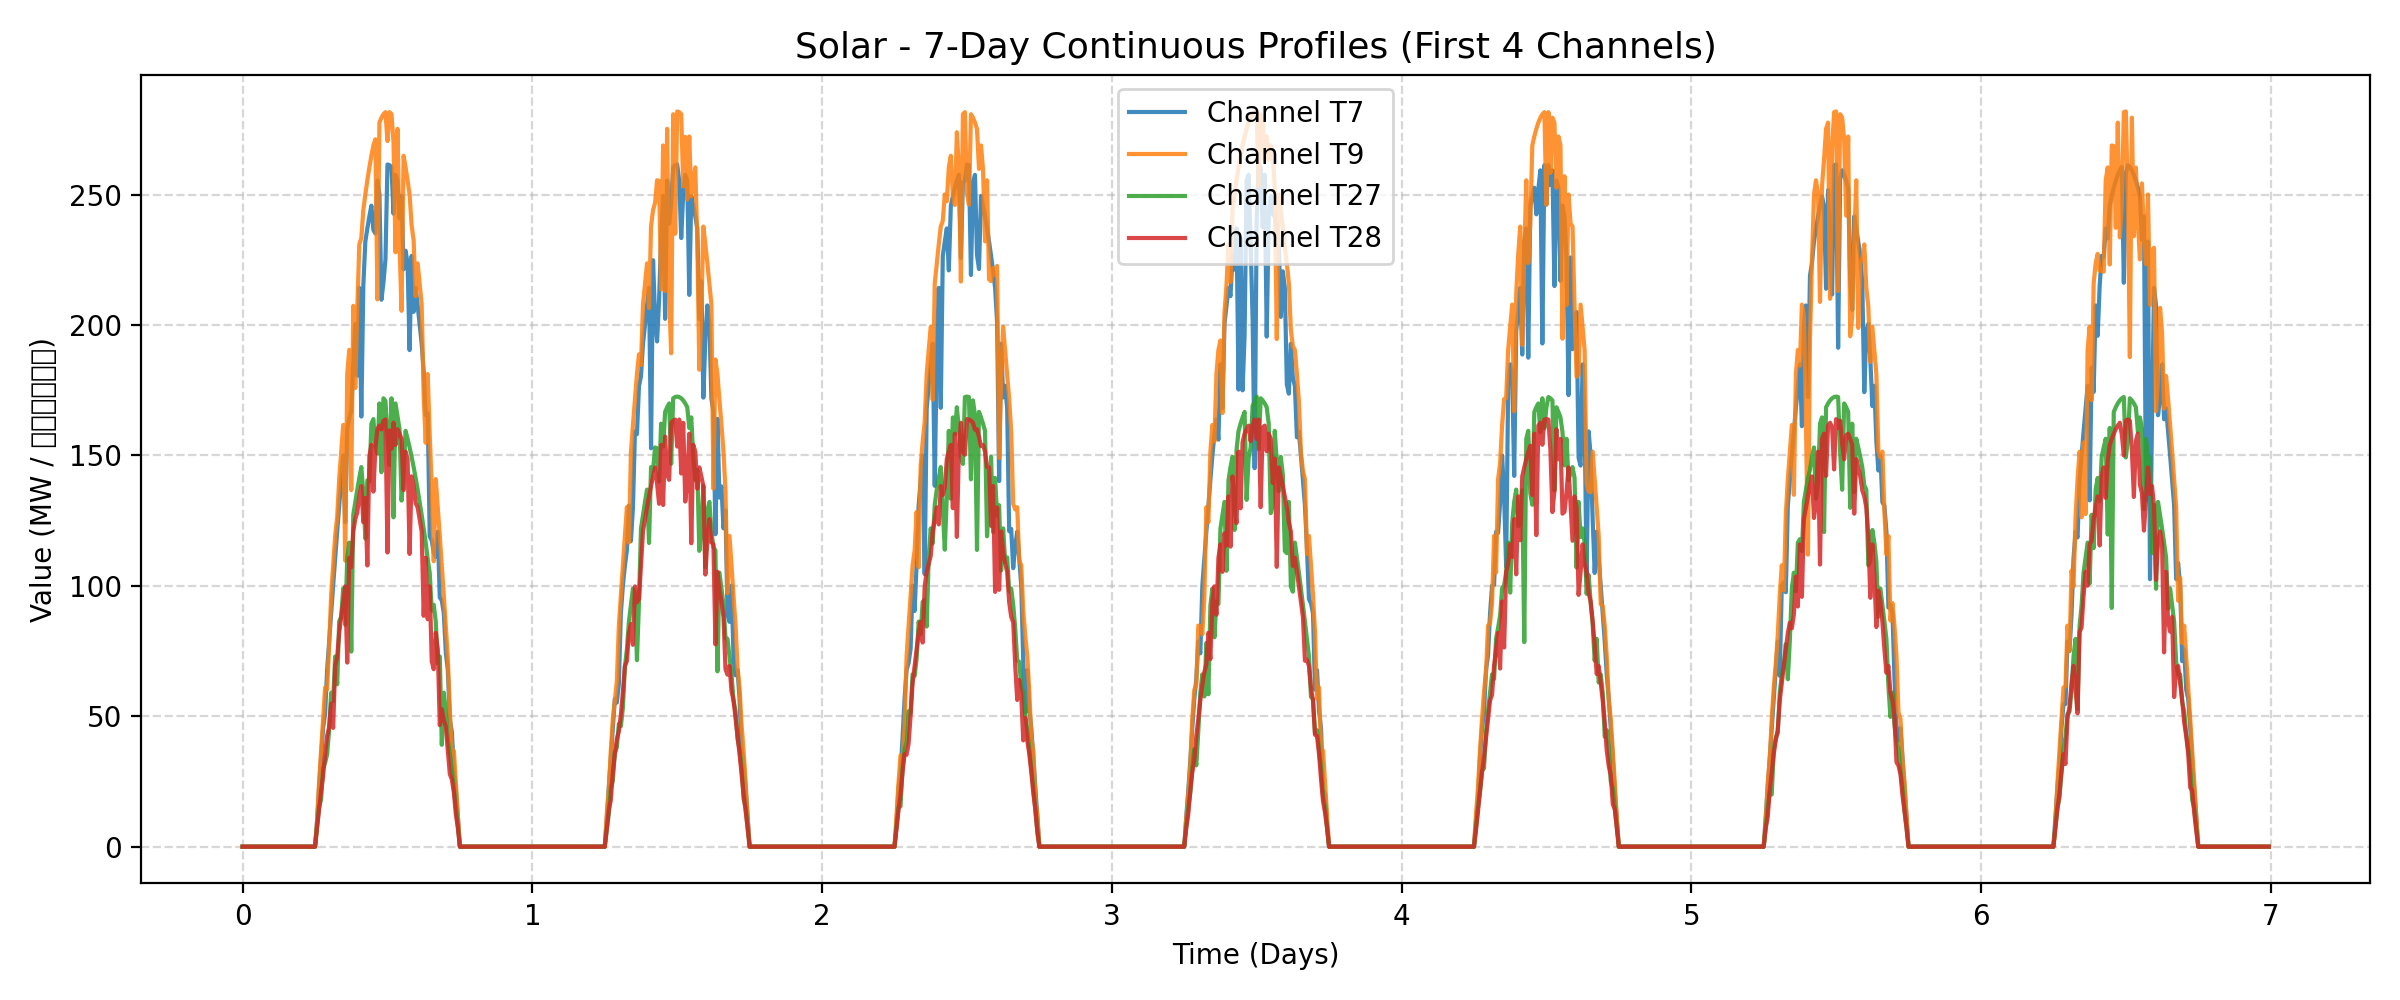
\includegraphics[width=\textwidth]{figures/solar_7day_profile.png}
        \caption{Solar: 7-Day Continuous Output Profile}
        \label{fig:solar_eda}
    \end{subfigure}
    \caption{Continuous 7-day trajectories demonstrating distinct diurnal regimes and zero-night solar properties.}
    \label{fig:eda_profiles}
\end{figure}

\section{Initial Experimental Results and Comparative Analysis}
\label{sec:results}
\noindent\textit{[Author: Student 1]}

Tables~\ref{tab:results_elec} and~\ref{tab:results_solar} summarize initial benchmarking results obtained across both datasets under identical experimental conditions.

\begin{table}[H]
\centering
\small
\caption{Initial Forecasting Performance on Electricity Hourly Dataset ($L=48, H=24, C=16$).}
\label{tab:results_elec}
\resizebox{\textwidth}{!}{%
\begin{tabular}{lcccccccc}
\toprule
\textbf{Model} & \textbf{MAE (24h)} & \textbf{RMSE (24h)} & \textbf{MASE (24h)} & \textbf{MAE (4h)} & \textbf{Params} & \textbf{Train (s)} & \textbf{Infer (ms)} & \textbf{Peak MAE} \\
\midrule
Persistence & $14.6178$ & $17.9119$ & $2.3443$ & $8.6452$ & $0$ & $0.00$ & $0.38$ & $18.4569$ \\
Seasonal Naive & $6.2295$ & $7.4336$ & $0.9990$ & $6.2228$ & $0$ & $0.00$ & $0.35$ & $6.3191$ \\
\midrule
LSTM & $2.6245$ & $3.2948$ & $0.4209$ & $2.6337$ & $45,952$ & $3.07$ & $1.34$ & $2.8508$ \\
GRU & $2.6524$ & $3.3335$ & $0.4254$ & $2.6732$ & $40,704$ & $10.23$ & $4.63$ & $2.8846$ \\
1D-CNN & $\mathbf{2.5864}$ & $\mathbf{3.2460}$ & $\mathbf{0.4148}$ & $2.6130$ & $401,568$ & $3.46$ & $1.54$ & $2.7218$ \\
CNN--LSTM & $2.5940$ & $3.2578$ & $0.4160$ & $\mathbf{2.5855}$ & $61,504$ & $4.31$ & $1.81$ & $\mathbf{2.7072}$ \\
DLinear & $2.7894$ & $3.5025$ & $0.4473$ & $2.8345$ & $\mathbf{2,352}$ & $\mathbf{1.34}$ & $\mathbf{0.97}$ & $2.8850$ \\
PatchTST & $2.5932$ & $3.2557$ & $0.4159$ & $2.5932$ & $76,056$ & $23.69$ & $3.95$ & $2.7250$ \\
\bottomrule
\end{tabular}%
}
\end{table}

\begin{table}[H]
\centering
\small
\caption{Initial Forecasting Performance on Solar 10-Minute Dataset ($L=288, H=144, C=16$).}
\label{tab:results_solar}
\resizebox{\textwidth}{!}{%
\begin{tabular}{lcccccccc}
\toprule
\textbf{Model} & \textbf{MAE (24h)} & \textbf{RMSE (24h)} & \textbf{MASE (24h)} & \textbf{MAE (4h)} & \textbf{Params} & \textbf{Train (s)} & \textbf{Infer (ms)} & \textbf{Active MAE} \\
\midrule
Persistence & $83.9599$ & $115.6596$ & $14.2416$ & $36.3267$ & $0$ & $0.00$ & $0.61$ & $105.3353$ \\
Seasonal Naive & $\mathbf{5.9095}$ & $13.8224$ & $\mathbf{1.0027}$ & $\mathbf{5.9060}$ & $0$ & $0.00$ & $0.51$ & $12.6383$ \\
\midrule
LSTM & $17.6741$ & $23.5373$ & $2.9960$ & $20.9072$ & $170,752$ & $3.70$ & $4.41$ & $20.4469$ \\
GRU & $15.1148$ & $19.4309$ & $2.5632$ & $16.8276$ & $165,504$ & $20.81$ & $23.59$ & $17.0085$ \\
1D-CNN & $9.1339$ & $\mathbf{12.9118}$ & $1.5502$ & $9.0650$ & $2,369,568$ & $3.92$ & $4.29$ & $12.2300$ \\
CNN--LSTM & $12.9477$ & $18.4266$ & $2.1974$ & $15.9990$ & $186,304$ & $5.62$ & $6.79$ & $17.6566$ \\
DLinear & $9.2211$ & $12.9778$ & $1.5656$ & $9.2554$ & $\mathbf{83,232}$ & $\mathbf{0.91}$ & $\mathbf{1.95}$ & $\mathbf{12.2175}$ \\
PatchTST & $10.3210$ & $14.5301$ & $1.7517$ & $10.0440$ & $392,976$ & $68.55$ & $38.50$ & $13.0294$ \\
\bottomrule
\end{tabular}%
}
\end{table}

\begin{figure}[H]
    \centering
    \begin{subfigure}[b]{0.48\textwidth}
        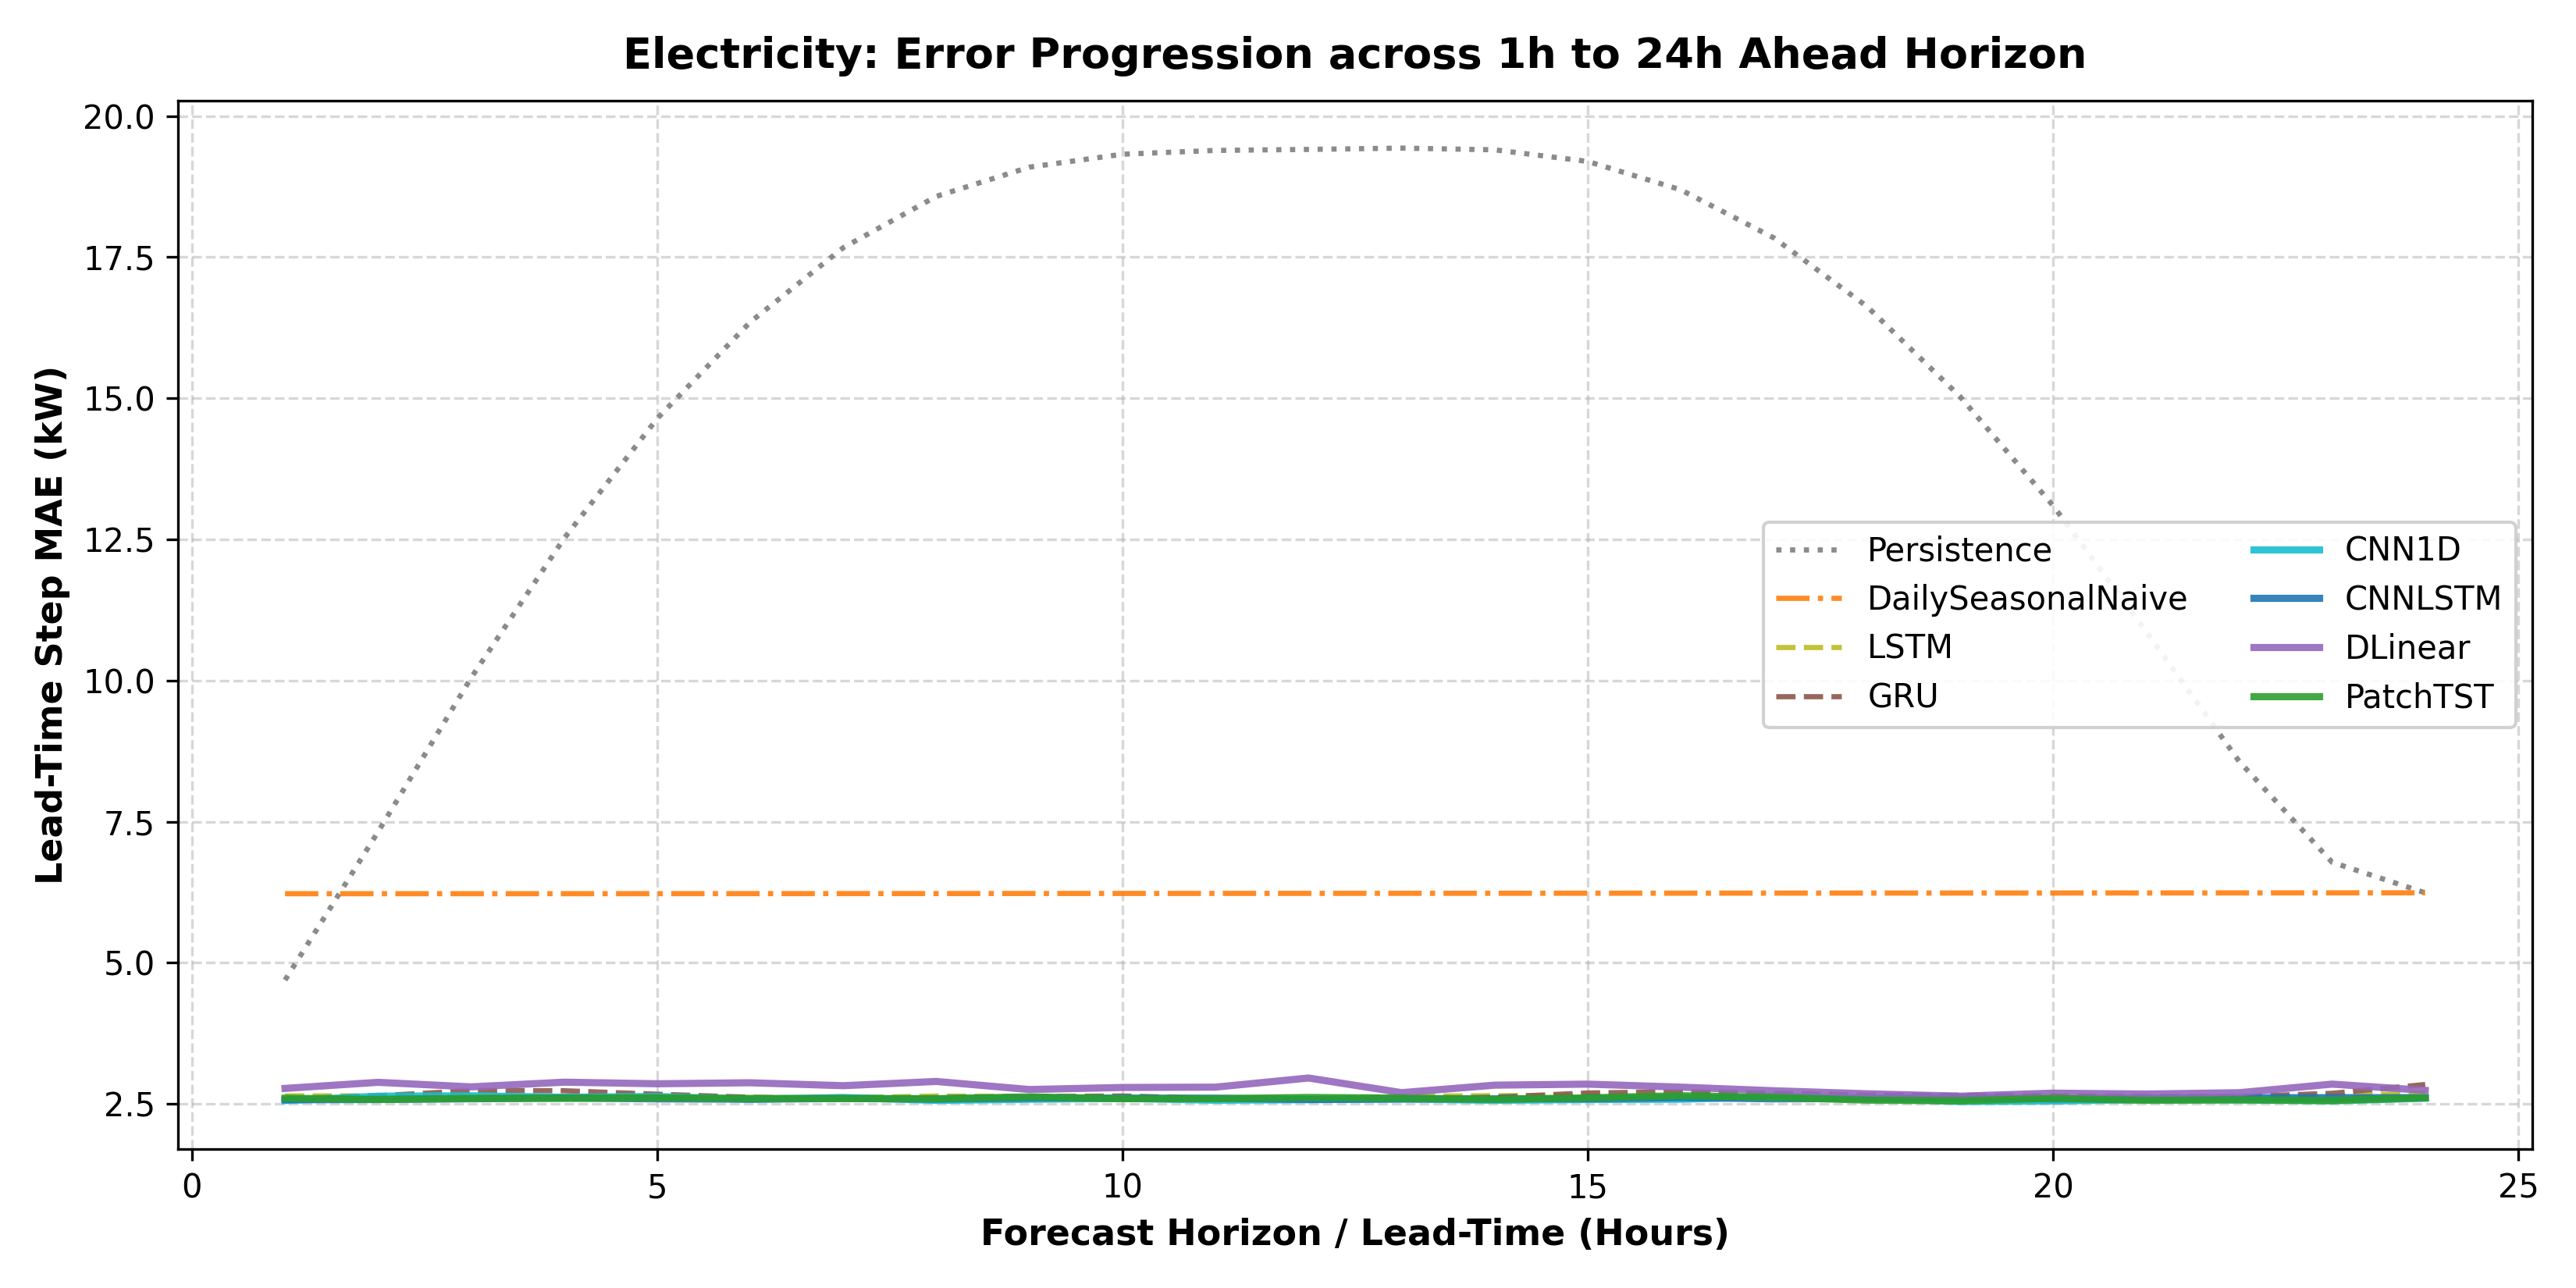
\includegraphics[width=\textwidth]{figures/lead_time_curves_electricity.png}
        \caption{Electricity Lead-Time Error Curves}
        \label{fig:lt_elec}
    \end{subfigure}
    \hfill
    \begin{subfigure}[b]{0.48\textwidth}
        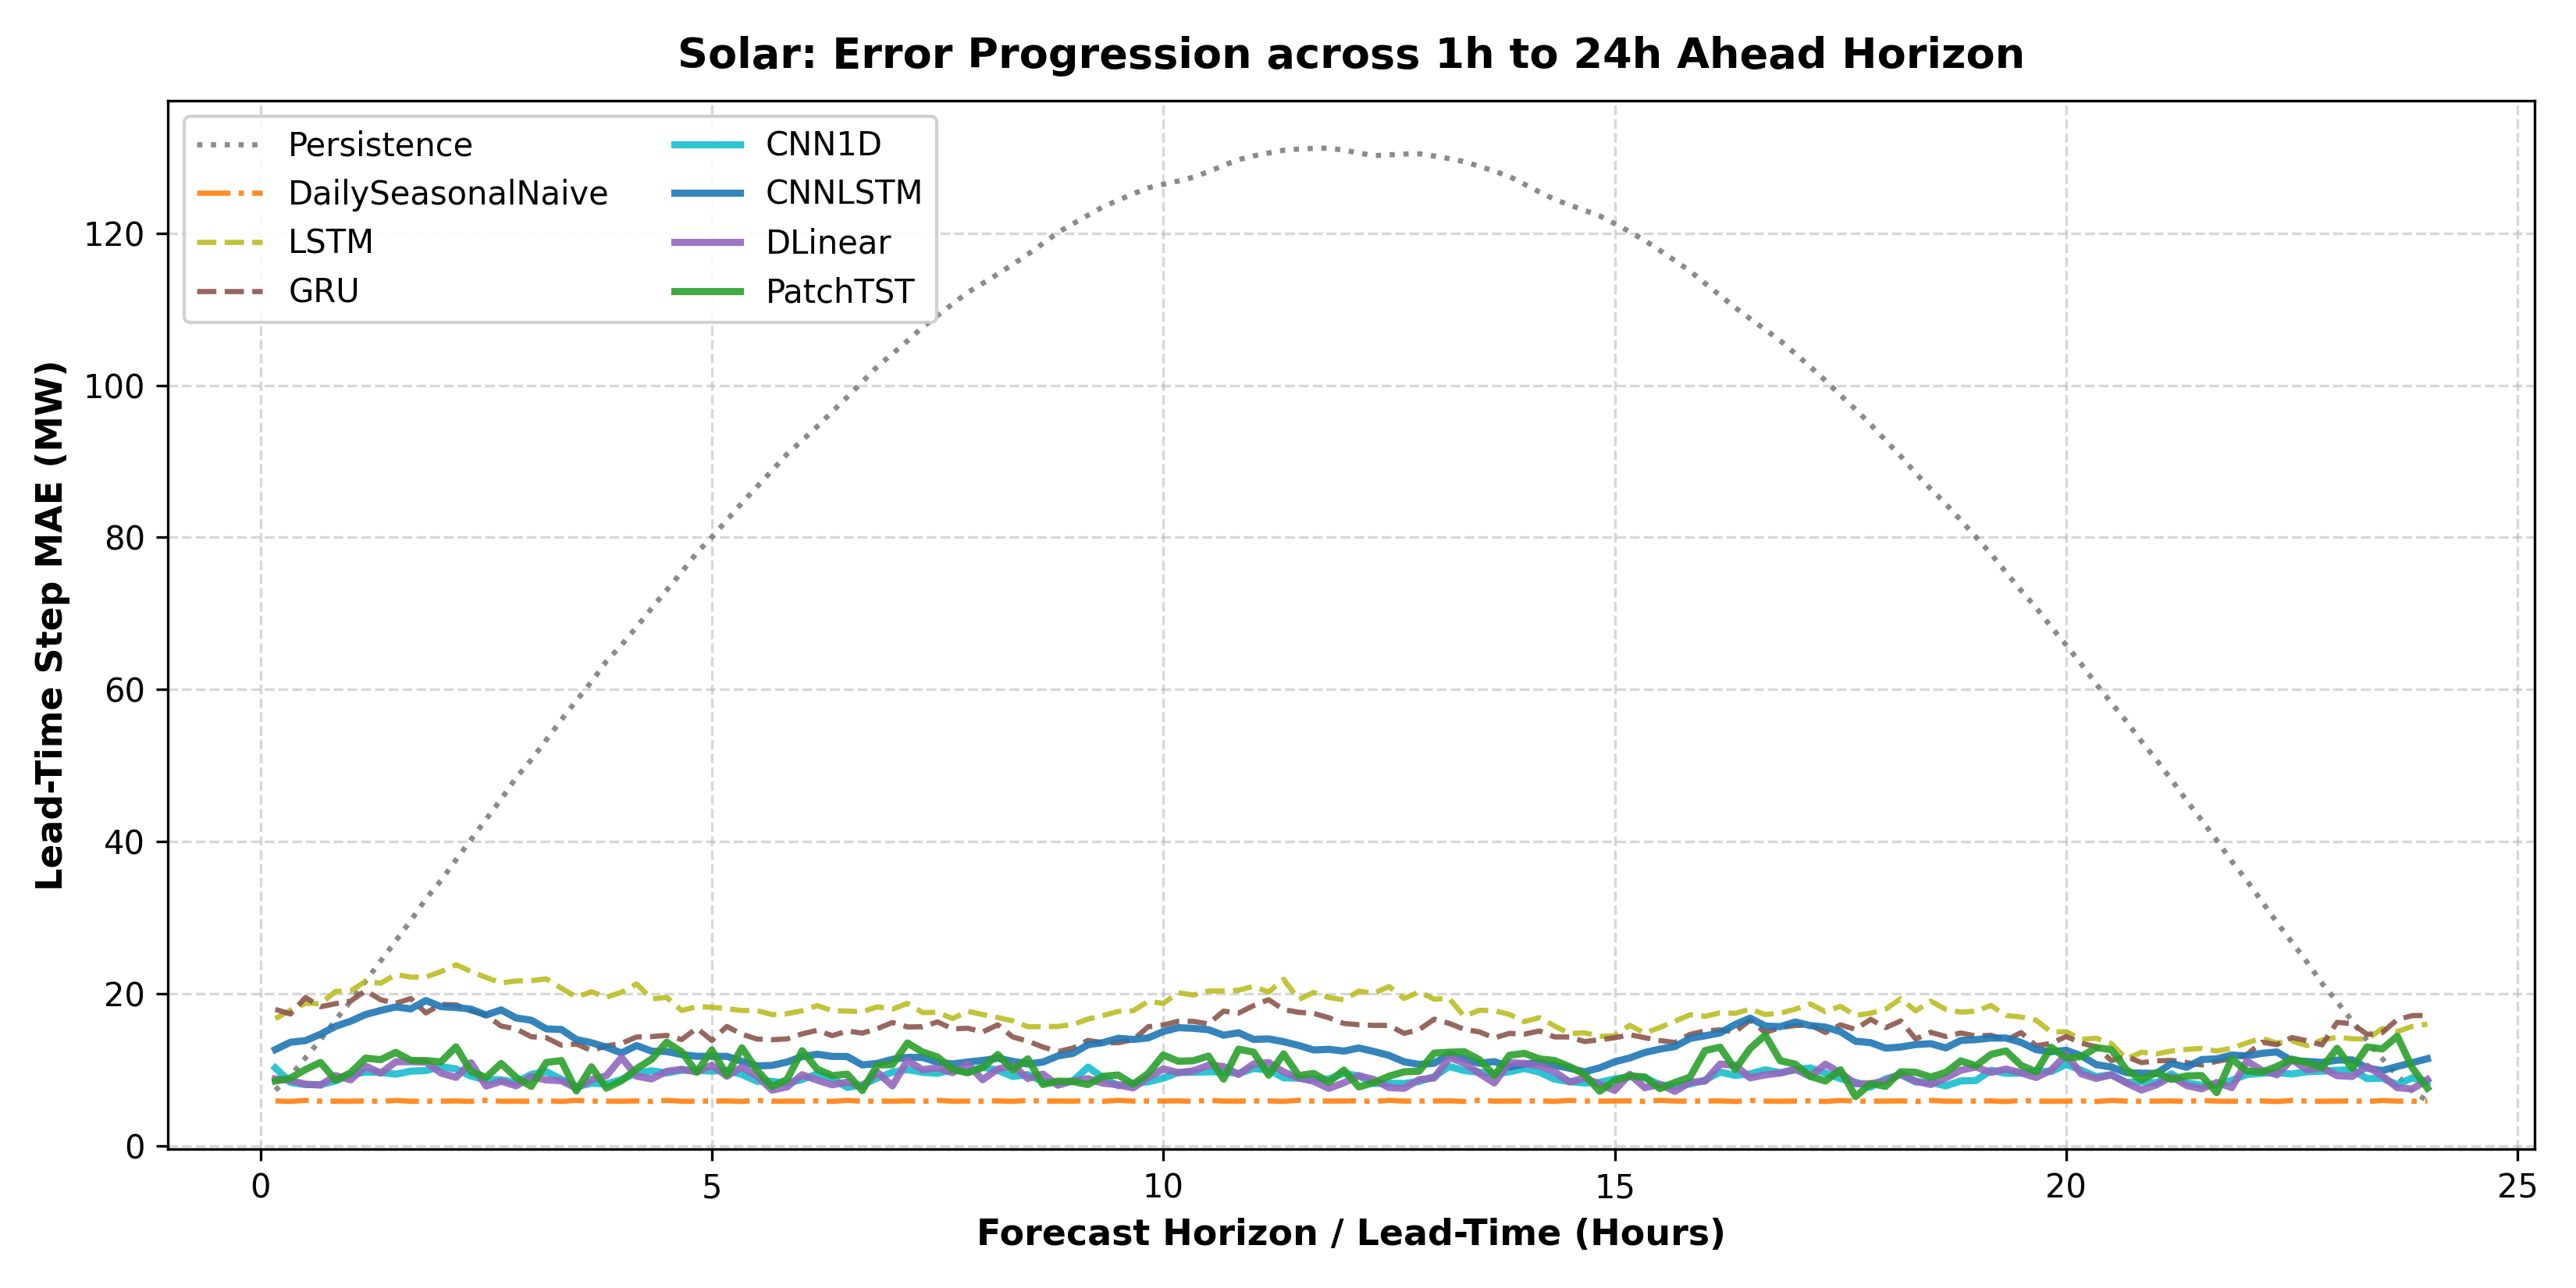
\includegraphics[width=\textwidth]{figures/lead_time_curves_solar.png}
        \caption{Solar Lead-Time Error Curves}
        \label{fig:lt_solar}
    \end{subfigure}
    \caption{Error progression across the 24-hour horizon showing divergence in deep learning versus persistence methods.}
    \label{fig:lead_time}
\end{figure}

\begin{figure}[H]
    \centering
    \begin{subfigure}[b]{0.48\textwidth}
        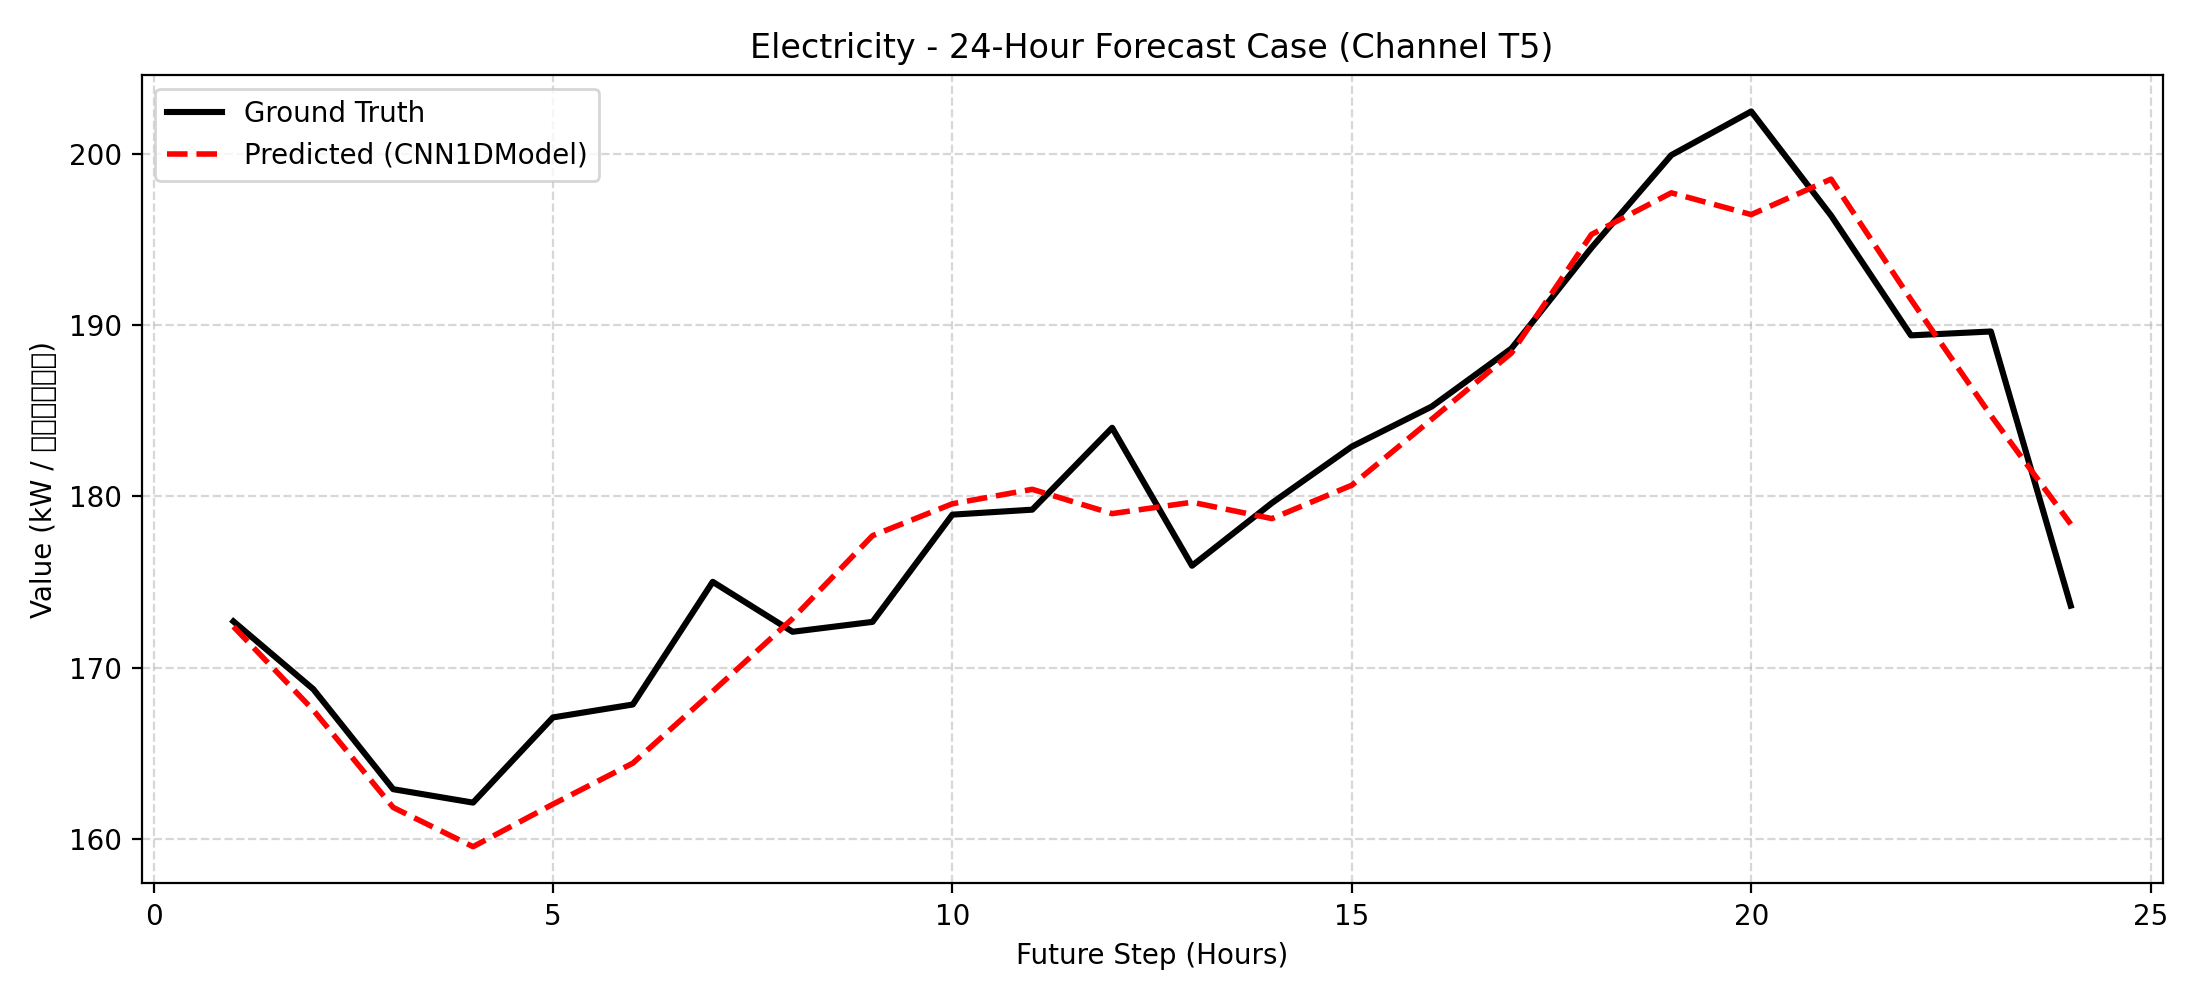
\includegraphics[width=\textwidth]{figures/forecast_case_electricity.png}
        \caption{Electricity: 24h Prediction Trajectory vs Ground Truth}
        \label{fig:case_elec}
    \end{subfigure}
    \hfill
    \begin{subfigure}[b]{0.48\textwidth}
        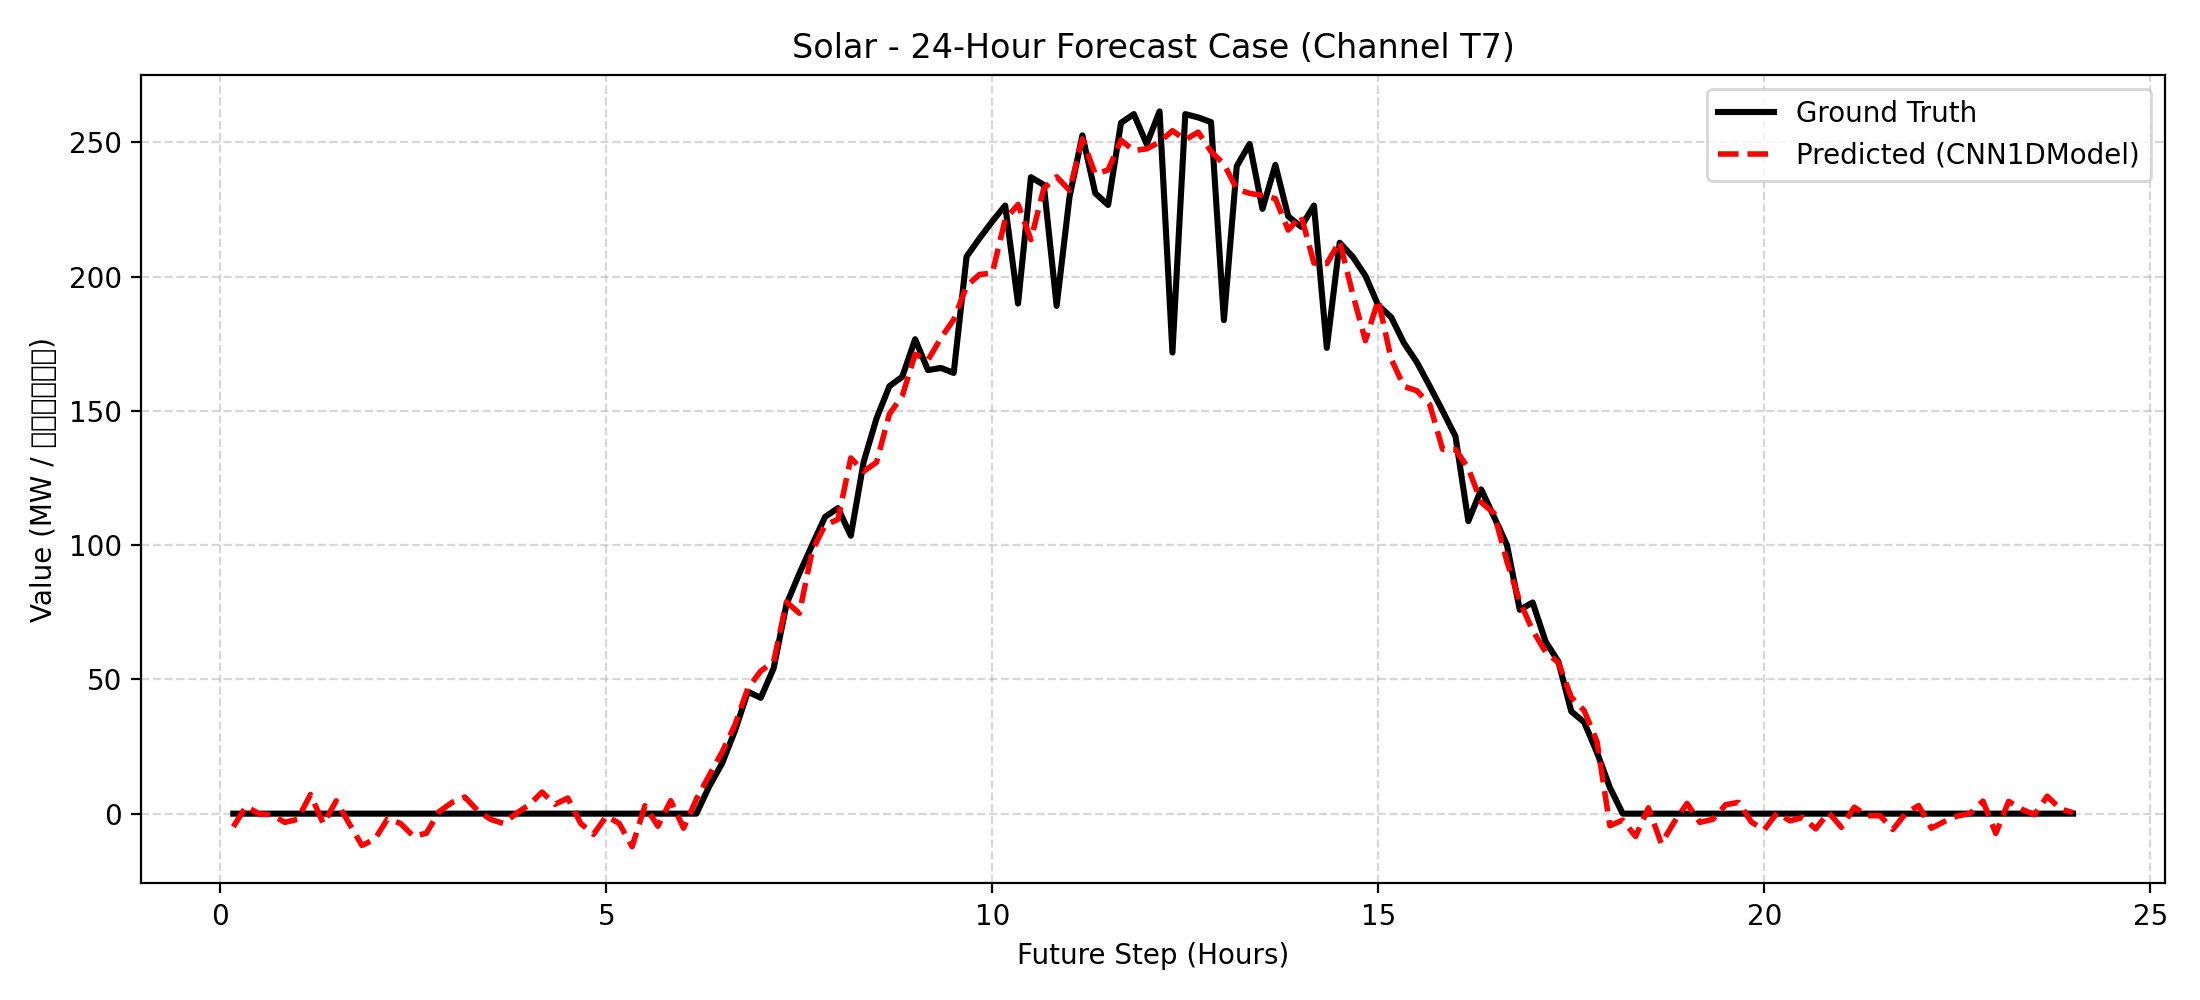
\includegraphics[width=\textwidth]{figures/forecast_case_solar.png}
        \caption{Solar: 24h Prediction Trajectory vs Ground Truth}
        \label{fig:case_solar}
    \end{subfigure}
    \caption{Representative 24-hour test forecast instances demonstrating model tracking of peak consumption cycles and night-time zero solar output.}
    \label{fig:forecast_cases}
\end{figure}

\subsection{Key Empirical Insights}
\begin{enumerate}
    \item \textbf{Significant Deep Learning Gains in Electricity:} On electricity demand, all deep learning models achieve outstanding performance, reducing MASE from $0.9990$ (Seasonal Naive) to $\approx 0.415$ (1D-CNN, PatchTST, and CNN--LSTM). This corresponds to a dramatic $58.4\%$ reduction in forecast error.
    \item \textbf{Solar Night-Zero Dominance:} On solar power, Daily Seasonal Naive achieves a competitive MAE of $5.9095$ primarily because nocturnal zero generation constitutes nearly half of all daily observations. However, in daytime active generation slices, 1D-CNN ($12.23$) and DLinear ($12.21$) outperform Seasonal Naive ($12.63$), demonstrating their ability to filter intermittent cloud fluctuations.
    \item \textbf{The DLinear Pareto Frontier:} DLinear requires only $2,352$ parameters for Electricity (compared to $76,056$ for PatchTST and $401,568$ for 1D-CNN) while achieving an MAE of $2.7894$ with an ultra-low inference latency of $0.97$ ms. It represents the most computationally viable option for edge-deployed embedded power meters.
\end{enumerate}

\section{Sensitivity and Ablation Studies}
\label{sec:sensitivity}
\noindent\textit{[Author: Student 2]}

\subsection{Experiment A: Historical Window Length Sensitivity}
We investigate the impact of expanding historical observation lengths $L \in \{24, 48, 168\}$ hours on Electricity demand under identical forecast evaluation origins:
\begin{table}[H]
\centering
\small
\caption{Historical Window Length Sensitivity on Electricity Demand ($H=24$ Hours, Common Start Alignment $\text{common\_start\_idx}=168$).}
\label{tab:sens_window}
\resizebox{\textwidth}{!}{%
\begin{tabular}{lccccc}
\toprule
\textbf{Model} & \textbf{History Length ($L$)} & \textbf{MAE (24h)} & \textbf{RMSE (24h)} & \textbf{MASE (24h)} & \textbf{Training Time (s)} \\
\midrule
LSTM & $24$ Hours ($24$ steps) & $2.9234$ & $3.6947$ & $0.4688$ & $2.45$ \\
LSTM & $48$ Hours ($48$ steps) & $2.5588$ & $3.2134$ & $0.4104$ & $3.21$ \\
LSTM & $168$ Hours ($1$ Week) & $2.5538$ & $3.2079$ & $0.4096$ & $6.71$ \\
\midrule
PatchTST & $24$ Hours ($24$ steps) & $3.1506$ & $3.9843$ & $0.5053$ & $11.88$ \\
PatchTST & $48$ Hours ($48$ steps) & $2.5795$ & $3.2388$ & $0.4137$ & $23.35$ \\
PatchTST & $168$ Hours ($1$ Week) & $\mathbf{2.4751}$ & $\mathbf{3.1064}$ & $\mathbf{0.3969}$ & $94.52$ \\
\bottomrule
\end{tabular}%
}
\end{table}
As demonstrated in Table~\ref{tab:sens_window}, expanding the observation window from $24$h to $168$h (incorporating the full weekly cycle) steadily improves predictive accuracy. Most prominently, PatchTST achieves the best overall performance at $L=168$ ($\text{MASE}=0.3969$, a $21.5\%$ error reduction compared to $L=24$). For PatchTST, very short windows ($24$h) perform worse because $16$-step patching yields only two tokens, which restricts multi-head self-attention expressiveness.

\subsection{Experiment B: Training Data Volume Sensitivity}
To evaluate model stability under data scarcity, models are trained on $25\%$, $50\%$, and $100\%$ sub-samples of the training interval (anchored at $b_1$ and truncated backwards). 
\begin{table}[H]
\centering
\small
\caption{Training Data Volume Sensitivity on Electricity Demand ($L=48, H=24$).}
\label{tab:sens_datasize}
\resizebox{\textwidth}{!}{%
\begin{tabular}{lccccc}
\toprule
\textbf{Model} & \textbf{Data Fraction} & \textbf{MAE (24h)} & \textbf{RMSE (24h)} & \textbf{MASE (24h)} & \textbf{Training Time (s)} \\
\midrule
LSTM & $25\%$ & $5.7418$ & $7.0145$ & $0.9206$ & $1.09$ \\
LSTM & $50\%$ & $3.4468$ & $4.3278$ & $0.5523$ & $1.70$ \\
LSTM & $100\%$ & $2.6245$ & $3.2948$ & $0.4209$ & $3.07$ \\
\midrule
PatchTST & $25\%$ & $2.6789$ & $3.3621$ & $0.4295$ & $6.86$ \\
PatchTST & $50\%$ & $2.6265$ & $3.2957$ & $0.4208$ & $12.94$ \\
PatchTST & $100\%$ & $\mathbf{2.5932}$ & $\mathbf{3.2557}$ & $\mathbf{0.4159}$ & $23.69$ \\
\bottomrule
\end{tabular}%
}
\end{table}
As detailed in Table~\ref{tab:sens_datasize}, PatchTST exhibits remarkable sample efficiency: even with only $25\%$ training data, PatchTST degrades by merely $3.3\%$ ($0.4159 \to 0.4295$ MASE), outperforming even the full-data LSTM ($0.4209$). This resilience is attributed to its Channel Independence inductive bias, where all 16 channels share the same Transformer encoder weights, effectively providing a $16\times$ token multiplier during optimization. In contrast, standalone LSTM degrades sharply under $25\%$ data ($\text{MASE}=0.9206$), failing to converge on stable recurrent gating dynamics without extensive sample trajectories.

\subsection{Experiment C: Modular CNN Ablation in CNN--LSTM}
To isolate the specific contribution of the temporal convolutional frontend, we compare CNN--LSTM against its constituent components:
\begin{table}[H]
\centering
\small
\caption{Modular Convolutional Frontend Ablation on Electricity Demand ($L=48, H=24$).}
\label{tab:ablation_cnn}
\resizebox{\textwidth}{!}{%
\begin{tabular}{lccccc}
\toprule
\textbf{Architecture} & \textbf{MAE (24h)} & \textbf{RMSE (24h)} & \textbf{MASE (24h)} & \textbf{Params} & \textbf{Train Time (s)} \\
\midrule
Standalone LSTM & $2.6245$ & $3.2948$ & $0.4209$ & $45,952$ & $3.07$ \\
Standalone 1D-CNN & $\mathbf{2.5864}$ & $\mathbf{3.2460}$ & $\mathbf{0.4148}$ & $401,568$ & $3.46$ \\
Hybrid CNN--LSTM & $2.5940$ & $3.2578$ & $0.4160$ & $61,504$ & $4.31$ \\
\bottomrule
\end{tabular}%
}
\end{table}
Table~\ref{tab:ablation_cnn} confirms that prefixing temporal convolutions before the recurrent cell improves LSTM prediction accuracy from $2.6245$ to $2.5940$ MAE. Temporal convolutions extract localized intra-day wavelets, relieving the recurrent state from memorizing high-frequency fluctuations. Furthermore, CNN--LSTM achieves this with only $61,504$ parameters, offering an $84.7\%$ parameter reduction compared to pure 1D-CNN ($401,568$ parameters).

\section{Discussion, Limitations, and Project Roadmap}
\label{sec:discussion}
\noindent\textit{[Author: Student 1 \& Student 2]}

\subsection{Current Limitations}
\begin{itemize}
    \item \textbf{Absence of Exogenous Weather Regressors:} All models rely solely on past target loads. Real-world solar forecasting relies heavily on numerical weather prediction (irradiance, cloud index, ambient temperature).
    \item \textbf{Single Temporal Fold:} Results are evaluated on a single chronological test window; rolling backtesting over multiple seasonal folds will solidify statistical confidence.
\end{itemize}

\subsection{Roadmap Toward Final Submission}
\begin{enumerate}
    \item Execute multi-seed runs ($3$ seeds) across all architectures to report mean and standard deviations.
    \item Implement vector-database retrieval exploration for historical analog matching as suggested in the course guidelines.
    \item Refine hyperparameter tuning (learning rate scheduling, dropout rates) using only the validation partition.
    \item Conduct detailed residual error decomposition and failure mode analysis on severe extreme weather days.
\end{enumerate}

\bibliographystyle{IEEEtran}
\begin{thebibliography}{10}

\bibitem{box2015time}
G.~E. Box, G.~M. Jenkins, G.~C. Reinsel, and G.~M. Ljung, \emph{Time Series Analysis: Forecasting and Control}.\hskip 1em plus 0.5em minus 0.4em\relax John Wiley \& Sons, 2015.

\bibitem{zhang2014review}
Y.~Zhang, J.~Wang, and X.~Wang, ``Review on probabilistic forecasting of wind power generation,'' \emph{Renewable and Sustainable Energy Reviews}, vol.~32, pp. 255--270, 2014.

\bibitem{hochreiter1997long}
S.~Hochreiter and J.~Schmidhuber, ``Long short-term memory,'' \emph{Neural Computation}, vol.~9, no.~8, pp. 1735--1780, 1997.

\bibitem{cho2014learning}
K.~Cho, B.~van Merri{\"e}nboer, {\c{C}}.~G{\"u}l{\c{c}}ehre, D.~Bahdanau, F.~Bougares, H.~Schwenk, and Y.~Bengio, ``Learning phrase representations using {RNN} encoder-decoder for statistical machine translation,'' in \emph{EMNLP}, 2014, pp. 1724--1734.

\bibitem{zeng2023transformers}
A.~Zeng, M.~Chen, L.~Zhang, and Q.~Xu, ``Are transformers effective for time series?'' in \emph{Proceedings of the AAAI Conference on Artificial Intelligence}, vol.~37, no.~9, 2023, pp. 11\,121--11\,128.

\bibitem{nie2023time}
Y.~Nie, N.~H. Nguyen, P.~Sinthong, and J.~Kalagnanam, ``A time series is worth 64 words: Long-term forecasting with transformers,'' in \emph{International Conference on Learning Representations (ICLR)}, 2023.

\bibitem{godahewa2021monash}
C.~Godahewa, C.~Bergmeir, G.~I. Webb, R.~J. Hyndman, and P.~Montero-Manso, ``Monash time series forecasting repository,'' in \emph{NeurIPS Datasets and Benchmarks Track}, 2021.

\bibitem{hyndman2006another}
R.~J. Hyndman and A.~B. Koehler, ``Another look at measures of forecast accuracy,'' \emph{International Journal of Forecasting}, vol.~22, no.~4, pp. 679--688, 2006.

\end{thebibliography}

\end{document}
